\chapter{JSCsim: A Joint Source--Channel Coding Simulator}
\label{ch:simulator}

\DefineShortVerb{\|}


\section[Object Oriented Programming for Simulations]{Object Oriented
Programming and Simulation: A Great Match}\label{sec:ooforsim}

\subsection{The ``Traditional'' Way}

Imagine that you have written the code in \lstref{proceduralsim} to simulate
your recently devised communication scheme. The function |run_simulation()|
first defines a few relevant parameters and creates a vector of random source
samples. Then, for each SNR value in the defined range, it calls |encode()| to
encode the source symbols into the channel input~|x|, adds noise, decodes the
result~|y|  to produce an estimate~|sh|.  Finally it computes the empirical MSE
and stores it in the vector~|mse|.

\begin{listing}
\begin{Code}
  function mse = run_simulation()
    snr = 10.^(0:.1:5);   % SNR range: 0 to 50 dB
    sv  = 1;              % Source variance
    N   = 100000;         % Sample size
    
    s = get_source_samples(N, sv);
    for k = 1:length(snr)
      x  = encode(s);
      y  = x + gaussian_noise(snr(k));
      sh = decode(y);
      
      mse(k) = mean((s - sh).^2);
    end
  end
\end{Code}
\caption{A hypothetical simulation of a joint source-channel communication
scheme.}
\label{lst:proceduralsim}
\end{listing}

Suppose now that you want to test an alternative decoding method. For example,
you want to see how a maximum likelihood decoder compares to an MMSE decoder. To
this end you write the function |alt_decode()|. How do you test this function?
You have essentially three possibilities:
\begin{enumerate}
  \item You replace the call to |decode()| in |run_simulation()| by a call to
    |alt_decode()|. The change to the existing code is only minimal. In doing
    so, however, you lose the old code, which is not very good since you
    probably would like to compare the performance of the new decoder to that of
    the old one. 

  \item You copy the contents of |run_simulation()| into a new function called
    |run_alt_simulation()|, replacing the call to |decode()| with a call to
    |alt_decode()|. While
    this approach leaves the old code unchanged and again only requires a small
    programming effort, it results in a lot of duplicate code, which makes your
    program error prone.

  \item You do as in point~2, but then you eliminate duplicate code by putting
    all the common code into separate functions that will be called by both
    |run_simulation()| and |run_alt_simulation()|. This does indeed remove the
    redundancies, but it also requires significant programming effort. Moreover,
    if one day you decide to change the encoder as well, this will probably
    again require a similar amount of effort. 
\end{enumerate}

As you can see, none of these options is quite satisfactory. You either lose old
functionality, are left with a lot of duplicate code, or face a significant
restructuring effort.


\paragraph{The Power of Inheritance}

Suppose now that your programming language supports object-oriented programming
and that you have implemented |run_simulation()| as a \emph{method} (or
\emph{member function}) of the class |Simulation|, as shown in
\lstref{objectsim}. Creating a new simulation with an alternative |decode()|
function now couldn't be easier: just create a \emph{derived class}\footnote{In
many languages, derived classes are called \emph{subclasses} and base classes
are called \emph{superclasses}. As pointed out by
Stroustrup~\cite{Stroustrup1997}, this is somewhat confusing because the
capabilities of a \emph{sub}class form a \emph{super}set of those of its
superclass (and vice versa). Hence in this text we shall stick to the terms
\emph{base class} and \emph{derived class}.} of |Simulation| and override the
|decode()| method, as shown in \lstref{derivedclass}. 

\begin{listing}
\begin{Code}
  classdef Simulation
    methods
      function mse = run_simulation()
        ... % as before
      end

      function x = encode(s)
        ...
      end

      function sh = decode(y)
        ...
      end
    end
  end
\end{Code}
  \caption{Object-oriented version of the simulator of \lstref{proceduralsim}.}
  \label{lst:objectsim}
\end{listing}

\begin{listing}
\begin{Code}
  classdef AlternativeSimulation < Simulation
    methods
      function sh = decode(y)
        % Alternative decoder implementation.
      end
    end 
  end
\end{Code}
  \caption{A new simulation with an alternative decoder is easily implemented by
  deriving a new class from \texttt{Simulation} and overriding the
  \texttt{decode()} function.}
  \label{lst:derivedclass}
\end{listing}

The object-oriented approach has none of the drawbacks of the previous example:
\begin{itemize}
  \item The original simulation remains completely unchanged.
  \item There is no programming effort other than implementing the new method.
  \item There is no redundant code whatsoever.
\end{itemize}

The concept we have exploited is called \emph{inheritance}, since
|Alternative|\-|Simulation| \emph{inherits} all those functions from
|Simulation| which it doesn't explicitly redefine.  The real power of
inheritance (at least for writing
simulations) is that it \emph{allows old code to call new code}: the
``old'' function |run_simulation()| calls the new |decode()| function, without
the need to make \emph{any} changes to the former. 

In classical \emph{procedural programming}, it is only possible for
\emph{new code to call old code}: a new function can call an existing one, but
the opposite is not possible without changing the existing function.
Furthermore, if you want two versions of an existing functions to coexist, such
that one of them calls a new function, this either causes code duplication
(which leads to bugs) or requires significant programming effort. 

To summarize, the simple act of  embedding a set of functions in a class and
then creating a derived class that overrides some of these functions created two
simulations that are identical except in a single function. 


\section{A Step-By-Step Tutorial}

\paragraph{Implementing a Simple Communication Scheme}

\exref{gausssingle} of \chapref{prelim} showed that uncoded transmission is
optimal to transmit a Gaussian source across a Gaussian channel if the source
and channel bandwidths are matched. To verify this claim experimentally, let us
implement \exref{gausssingle} in \jscsim. 

\begin{listing}
  \caption{Implementation of uncoded transmission.}
  \label{lst:uncoded}
  \CodeInput{simulator/@UncodedScheme/UncodedScheme.m}
\end{listing}

The code for this is shown in \lstref{uncoded}.  One can make the following
observations.
\begin{enumerate}
  \item The communication scheme is implemented as a \emph{class}, here called
    |Uncoded|\-|Scheme|. It is derived from the class |PracticalScheme|. This is
    the class that all ``practical'' communication schemes are derived from,
    \ie,
    communication schemes that can be implemented in practice as opposed to
    merely ``theoretical'' schemes (of which we will soon see an example).

  \item The constructor of |PracticalScheme| receives two parameters. |sv| is
    the source variance and |s| is the sequence of source symbols that are to be
    transmitted.\footnote{If you wonder why the constructor returns something
    called \Verb+obj+: this is simply how \matlab's syntax specifies the
    constructor.  The returned value stands for the object just created, and it
    serves as a ``pointer'' to access the object's properties, similar to the
    \Verb+this+ keyword in C++ or Java.}

    The constructor of the base class |PracticalScheme| needs two additional
    parameters. They are, respectively, the number~$k$ of source symbols encoded
    at a time and the number~$n$ of channel inputs produced from every
    $k$~source symbols. The scheme at hand is for the particular case when~$k =
    n = 1$, which is why the last two parameters passed to |PracticalScheme()|
    are both~$1$.

  \item The actual work of the class is done by the functions |encode()| and
    |decode()|. Any class derived from |PracticalScheme| \emph{must} implement
    these functions. Here they simply compute $X = \sqrt{P/\ssq} S$ and $\Sh =
    \sqrt{P \ssq} Y / (P + \szq)$.
\end{enumerate}


\paragraph{Performance Analysis}

Having implemented the class |UncodedScheme|, the next thing one might like to
do is to plot the resulting performance. This task is much simplified by the
class |Performance|\-|Processor|, which is used as follows.
\CodeInput{figures/matlab/ex_uncoded.minc}
The first two lines define two cell arrays with each a single entry.
The first contains the class names of the schemes to plot, and
the second contains a list of parameters for each scheme. Here we only have a
single scheme, |UncodedScheme|. It does not have any parameters, so the
corresponding entry in the parameter list is an empty vector. 

The third line creates an instance of the class |Performance|\-|Processor|, whose
|plot_performance()| method is invoked in the fourth line, specifying the
relevant schemes and parameters. The resulting plot is shown on
\figref{uncoded}.

\begin{figure}
  \begin{center}
    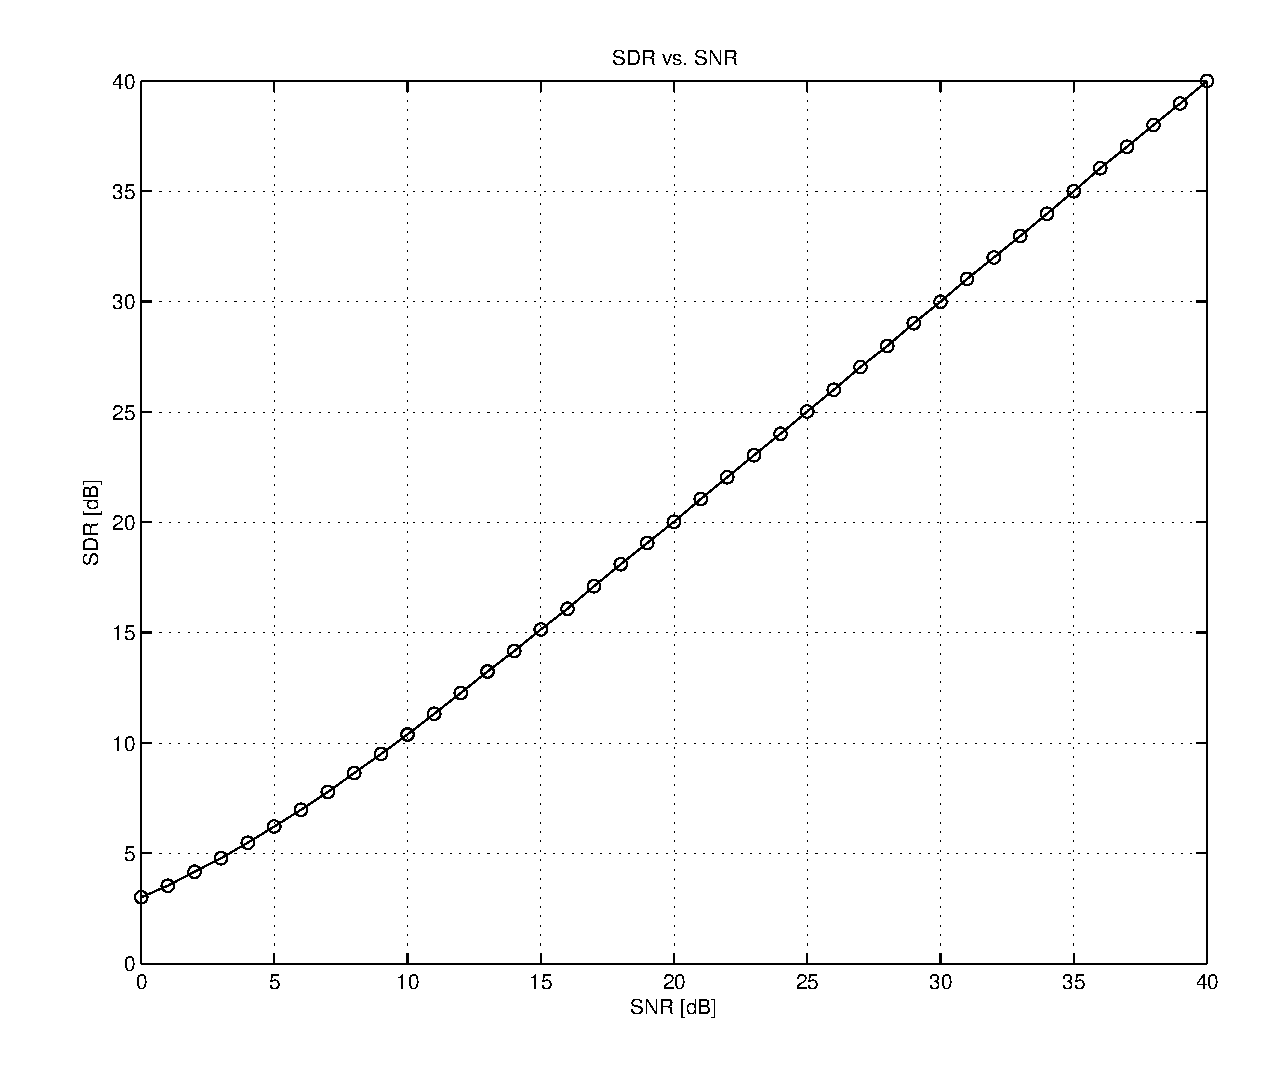
\includegraphics[width=\textwidth]{figures/matlab/ex_uncoded.pdf}
  \end{center}
  \caption{Plot of the SDR resulting from the \texttt{UncodedScheme} class,
  obtained using a \texttt{PerformanceProcessor}.}
  \label{fig:uncoded}
\end{figure}

This looks like not much at all. Behind the scenes, however, a lot more was
going on:
\begin{enumerate}
  \item A long sequence of random source symbols was generated.
  \item For a range of SNR values and for each communication scheme, the source
    sequence was encoded using the communication scheme, Gaussian noise of the
    appropriate variance was added, and the result was decoded using the
    scheme's |decode()| function.
  \item The average difference between the source sequence and the estimate
    sequence was computed, again for each scheme and for each value of SNR. 
  \item The resulting performance curves were plotted by |plot_performance()|.
\end{enumerate}
All this work is done by |Performance|\-|Processor| and the base class
|Practical|\-|Scheme|, leaving you free to focus on the essential stuff.


\paragraph{Theoretical Performance}

At this point we have implemented uncoded communication, but we have not
yet verified that it performs indeed optimally. From \chapref{prelim} we know
that if there are $n$~channel uses per source symbol then the optimal SDR
is $(1 + \snr)^n$. In \jscsim\ we can implement this as a ``theoretical''
communication scheme: this is a communication scheme that doesn't actually do
any encoding or decoding, but simply returns the achieved MSE for a given SNR.

\begin{listing}
\begin{Code}
  classdef ShannonScheme < Scheme
    properties
      n         % The number of channel uses per source symbol.
    end

    methods
      function obj = ShannonScheme(sv, s, n)
        
        % Call base class constructor.
        obj = obj@Scheme(sv, s);

        % Set class-specific parameters.
        obj.n = n;
      end

      % This function simply returns the theoretically optimal MSE
      % for the SNR.
      function mse = compute_mse(obj)
        mse = obj.sv / (1 + obj.snr)^obj.n;
      end
    end
  end
\end{Code}
  \caption{A ``theoretical'' communication scheme does not perform any
  actual encoding or decoding, but rather computes the theoretically optimal MSE
  for a given SNR.}
  \label{lst:shannonscheme}
\end{listing}

The resulting \matlab\ code is given in \lstref{shannonscheme}. We can make the
following observations.
\begin{enumerate}
  \item The class |ShannonScheme| is derived from |Scheme| rather than from
    |PracticalScheme| as in the previous example. This is because unlike
    practical schemes, |ShannonScheme| does not implement |encode()| or
    |decode()| functions. 
    
    |Scheme| is the class from which all communication schemes are derived. Each
    class derived from |Scheme| must implement |compute_mse()|, which returns
    the mean squared error obtained for a given SNR. In the previous example we
    did not have to implement this function because it is implemented by
    |PraticalScheme|, itself derived from |Scheme|.
    
  \item |ShannonScheme| has a single parameter, namely the number~|n| of channel
    uses per source symbol.

  \item The function |compute_mse(obj)| is the heart of this class. It computes
    the formula $\text{MSE} = \ssq / (1 + \snr)^n$. To access any of the class
    properties, their name must be prefixed by `|obj.|'.  Note in particular how
    |obj.snr| is accessed, even though it was never defined within this class.
    This is because it is handled by the base class. 
\end{enumerate}

To plot the performance of both |UncodedScheme| and |ShannonScheme|, we use
the |Performance|\-|Processor| as before:
\CodeInput{figures/matlab/ex_shannonscheme.minc}
The only difference to the previous exampe is that the list of schemes now has
an additional entry and we have to specify the parameter $n=1$ for
|ShannonScheme|.

The resulting plot is shown on \figref{shannonscheme}. Note that compared to
\figref{uncoded} we are plotting the performance of more than one communication
scheme here, so a legend was automatically added to the plot.

\begin{figure}
  \begin{center}
    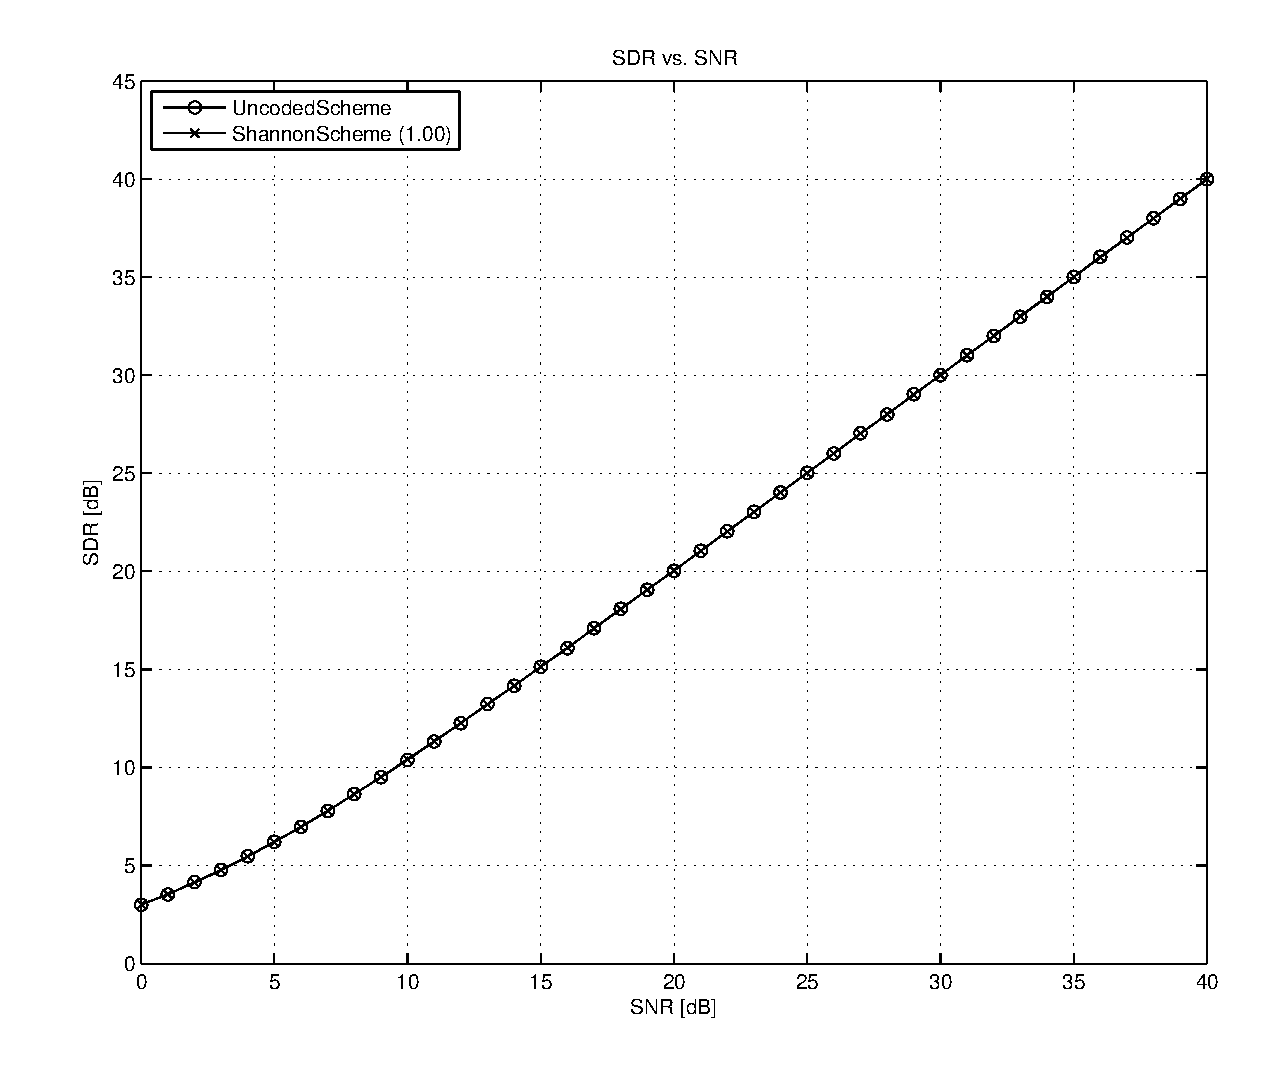
\includegraphics[width=\textwidth]{figures/matlab/ex_shannonscheme.pdf}
  \end{center}
  \caption{Comparing the theoretically optimal performance and the performance
  of uncoded transmission. The two curves coincide, experimentally confirming
  \exref{gausssingle}.}
  \label{fig:shannonscheme}
\end{figure}

\paragraph{Alternative Output Formats}

Up to now the call to |plot_performance()| just launched a standard \matlab\
figure window with the performance plot. Often, though, you may not only want to
look at the plot on the screen but also use it in a document such as a report or
a paper. For this, \jscsim\ has the concept of an \emph{output module}. An
output module implements a rudimentary set of plot capabilities. The default
output module uses \matlab's plot command to display a figure window.

Alternatively, to save the performance plot in a PDF file, for instance, the
default output module can be replaced by a |MatlabFilePlotModule|. Instead of
displaying the plot in a window, this module saves it in a file. Continuing our
previous example, we would use it as follows.
\begin{Code}
  ...  % Define list of schemes and parameters.
  pp = PerformanceProcessor();
  om = MatlabFilePlotModule();
  om.fn = 'myplot.pdf';
  pp.om = om;
  pp.plot_performance(schemes, parameters);  % Saved to myplot.pdf.
\end{Code}
In line~3 a new output module of type |MatlabFilePlotModule| is
created. Since it writes its output to a file, we have to specify a file name,
which we do in the next line. Finally, in the fourth line, we replace the
default output module of the performance processor with newly created
one.\footnote{Unsurprisingly, Figures~\ref{fig:uncoded}
and~\ref{fig:shannonscheme} have been created using
\Verb+MatlabFilePlotModule+.}

Another output module is called |PGFPlotsOutputModule|. It produces a file
containing \TeX\ code, to be used with the \pgfplots\ package. To use it, just
replace |MatlabFilePlotModule| in the above example by |PGFPlotsOutputModule|
and set \eg
\begin{Code}
  om.fn = 'myplot.tex';
\end{Code}
The resulting file can then be included in a \LaTeX\ file using the |\input|
command, provided that the |pgfplots| package has been loaded.  The result is
shown on \figref{uncodedpgf}. Admittedly, the plot created by \pgfplots\ fits in
nicer with the \LaTeX\ layout, and its labels are more readable than those of
Figures~\ref{fig:uncoded} and~\ref{fig:shannonscheme}.

\begin{figure}
  \begin{center}
    \input{figures/matlab/ex_uncodedpgf.tex_t}
  \end{center}
  \caption{Using the \texttt{PGFPlotsOutputModule}, one can save the simulation
  output as \TeX\ commands for the \pgfplots\ package, which can then be
  included in a \LaTeX\ source file.}
  \label{fig:uncodedpgf}
\end{figure}


\paragraph{Analysis Using Scheme Processors}

We have already seen one scheme processor in action. In the previous examples we
used a |Performance|\-|Processor| to plot the SDR resulting from different
communication schemes. |Performance|\-|Processor| is derived from the base class
|SchemeProcessor|. In general, a scheme processor takes a list of schemes (along
with the corresponding parameters), simulates these schemes for a range of SNR
values, and gathers particular data from each simulation run.  To illustrate
these principles, \lstref{perfproc} shows a simplified version of the
implementation of |Performance|\-|Processor|. 

\begin{listing}
\CodeInput{figures/matlab/PerformanceProcessor_ex.minc}
\caption{Simplified implementation of the \texttt{PerformanceProcessor} class.}
\label{lst:perfproc}
\end{listing}

Each class derived from |SchemeProcessor| must do three things:
\begin{enumerate}
  \item Call |set_schemes()| to store the list of schemes and the associated
    parameters.

  \item Call |process_schemes()|, the function that does the actual job of
    simulating each scheme for each SNR. |process_schemes()| is implemented in
    |SchemeProcessor|. 

  \item Implement |post_process()|. This function performs the ``data
    gathering''. It is called from within |process_schemes()| after each time a
    particular scheme has been simulated for a particular SNR. Its first
    argument |scheme| is the instance of the scheme just simulated. From it,
    |post_process()| can gather all required data.  In the case of
    |Performance|\-|Processor|, it simply queries the MSE and saves it in the
    |mse| matrix.
\end{enumerate}


Consider another example. Suppose we have a class |HybridScheme| that implements
the hybrid communication scheme from \textbf{[Insert reference to Ch.~2]}, and
suppose we would like to compare the errors $\Eqi$ and~$\Ee$. To do this, we would have |HybridScheme| store all $Q_i$ and
$\Qh_i$ as well as $E_{n-1}$ and $\Eh_{n-1}$. Then we could write a
|HybridSchemeProcessor| whose |post_process()| function computes and saves
$\Eqi$ and~$\Ee$. 


\section{Reference}

\subsection{Communication Schemes}

In \jscsim, there are two categories of communication schemes you can implement:
\emph{theoretical} schemes and \emph{practical} schemes. Theoretical schemes
merely compute the achievable MSE as a function of the SNR. Their purpose is to
allow you to compare the performance of a particular communication scheme with a
theoretical value, as for example the |ShannonScheme| in \lstref{shannonscheme}. 
On the other hand, practical schemes (like the one in \lstref{uncoded}) are
schemes that actually encode the source samples into a channel input sequence
and compute source estimates from the channel output. 

Theoretical and practical schemes, respectively, are implemented as classes
derived from |TheoreticalScheme| and |PracticalScheme|. The latter are
themselves derived from the common base class |Scheme|, which defines some of
the characteristics of both theoretical and practical communication scheme. 


\subsubsection{The \texttt{Scheme} Class}

In the class hierarchy, the |Scheme| class is the common ancestor of all classes
that implement communication schemes. It defines the characteristics shared by
all communication schemes, whether theoretical or practical (see previous
paragraphs). 

|Scheme| is an abstract class: no objects of this class can exist. Moreover,
there is usually no need to create a class derived directly from |Scheme| (other
than the existing |TheoreticalScheme| and |PracticalScheme|). Should there
nevertheless be a need for it, details about the implementation of |Scheme| are
found in the implementation section. 


\subsubsection{Theoretical Schemes}

Theoretical communication schemes are implemented as classes derived from
|TheoreticalScheme|. Any class derived from |TheoreticalScheme| must define the
following methods.

\begin{description}
  \item[\texttt{ClassName(sv, s, param)}] The first two arguments of the
    constructor are the source variance |sv| and the source sample sequence~|s|.
    For implementation purposes, they are passed to both theoretical and
    practical schemes. 

    The arguments |sv| and |s| must be passed on to the base class constructor.
    |param| is a parameter particular to the class to be implemented. It can be
    stored in a class property or processed as desired.

  \item[\texttt{update\_mse(obj)}] This function is called by the base class
    whenever the SNR is changed. It must update the |mse| property, based on the
    value of the |snr| property. For example, the |update_mse()| method of
    |ShannonScheme| sets |mse| to be $\ssq / (1 + \snr)^n$.
\end{description}


\subsubsection{Practical Schemes}

Practical communication schemes are implemented as classes derived from
|PracticalScheme|. Any class derived from |PracticalScheme| must define the
following methods.
\begin{description}
  \item[\texttt{Constructor(sv, s, param)}] The constructor of the class
    receives the source variance~|sv|, the source sample sequence~|s| and
    possibly a parameter |param|. The constructor must call the constructor of
    |PracticalScheme|, passing |sv| and |s| as well as |k| and |n|, the number
    of source symbols encoded at a time and the number of channel inputs per
    |k|~source symbols, respectively. 

    Depending on the scheme, |k| and |n| can be fixed values (as in
    |UncodedScheme| in \lstref{uncoded}) or they can be passed to the class as
    parameters.

  \item[\texttt{x = encode(obj, s)}] This function receives |s|, a matrix of
    source samples with |k|~rows, and must return a matrix~|x| with |n|~rows and
    the same number of columns as~|s|.

  \item[\texttt{sh = decode(obj, y)}] This function receives the channel
    output~|y| as a matrix with |n|~rows and must return a matrix~|sh| with
    |k|~rows of source estimates.
\end{description}


\subsection{Scheme Processors}

Usually you don't handle communication scheme classes directly; rather, you use
a \emph{scheme processor}. Scheme processors simulate a set of communication
schemes for a range of SNR values and let you store and process the resulting
data.  All scheme processors allow you to set the following properties, defined
in the base class |SchemeProcessor|.
\begin{description}
  \item[\texttt{snr}] This is a vector that specifies the SNR range over which
    to simulate the specified communication schemes. By default it is set to the
    range from 0dB to 40dB, with an increase of 1dB. 

  \item[\texttt{N}] This is the number of source samples generated. By default
    it is set to $10^5$. 
    
  \item[\texttt{verbose}] This is a boolean parameter. When set to true, various
    debugging and status messages are displayed during simulations. By default
    it is set to false. 

  \item[\texttt{om}] This is set to the output module used by the scheme
    processor to display its results (see the section on output modules). The
    default output module is |MatlabPlotModule|, which displays a standard
    \matlab\ plot.
\end{description}

To process a communication scheme (or a set of schemes) you never directly use
a |SchemeProcessor| object. Instead, you derive a new class from
|SchemeProcessor| that collects and processes the data of interest. One scheme
processor ``built into'' \jscsim\ is the |PerformanceProcessor|.

Each class derived from |SchemeProcessor| inherits the |process()| method from
|SchemeProcessor|. This is the only callable method; it is defined as follows. 
\begin{description}
  \item[\texttt{process(obj, schemes, parameters)}] Process the specified
    schemes for the specified parameters. |schemes| is a cell array of strings,
    each string being the name of a communication scheme class. Parameters is a
    cell array containg a vector for each element of |schemes|. For schemes that
    don't have any parameters, it must be an empty vector. Otherwise, the scheme
    is simulated separately for each parameter. 
\end{description}


\subsubsection{The Performance Processor}

This is the only scheme processor that is already implemented in \jscsim. It
works for all communication schemes derived from |Scheme|. It simply plots the
SDR vs SNR curve of the specified communication scheme. 


\subsubsection{Custom Scheme Processors}

You can implement your own scheme processor by creating a new class derived from
|SchemeProcessor|. Every such class must implement the following functions.
\begin{description}
  \item[\texttt{initialize(obj)}] This function is called before the actual
    processing of the schemes start. Most likely, you will use this function to
    allocate the matrices in which you will save the simulation data. 

    |SchemeProcessor| provides the useful helper function |nb_schemes()|, which
    returns the number of schemes that have been passed to |process()|. In
    addition, |length(obj.snr)| gives you the number of values in the SNR range.

  \item[\texttt{save\_scheme\_data(obj, scheme, j, k)}] This function is called
    each time a scheme has been simulated for a particular SNR and gives you the
    opportunity to save data about the simulation run. |scheme| is the scheme
    object that was just run; you can gather data about it by calling its public
    functions. For example, the |post_process()| method of
    |PerformanceProcessor| calls the |compute_mse()| method of the |scheme|
    object to store the MSE.

    To save a particular value for all schemes and all SNR values, you would
    normally create a big matrix with one row per scheme and parameter and one
    column for each SNR value. You can then use the indices |j| and |k| to know
    where to save a particular value in this matrix: |j| is an index into the
    list of all schemes processed and |k| is an index into the SNR range.

  \item[\texttt{post\_process(obj, scheme, j, k)}] This function is called after
    all the simulations have run. Here you can post process the data gathered by
    |save_scheme_data()|, for instance by plotting it.

    |SchemeProcessor| provides the useful function |plot_vs_snr(obj, m)|, which
    creates a plot of the data in the vector |m| against the SNR in dB, or
    several plots if |m| is a matrix with several rows. (The SNR is in dB, not
    the data; if you also want the data to be plotted in a dB scale you can use
    |plot_vs_snr_db()| instead.)
\end{description}


\subsection{Output Modules}

In some cases you might just want to see the results of a simulation on screen;
in other cases you might want to save them in a file that you can include in a
paper or report. In \jscsim\ it is easy to switch between the two options by
changing output modules.

Output modules provide an abstraction of basic plot functionalities. You can
think of them as a kind of output ``plugins''. The functionality they offer is
rather orthogonal to the task of simulating; you might use them in other
programs as well. 

In \jscsim, each class derived from |SchemeProcessor| has an output module
associated to it. By default this is the |MatlabPlotModule|, which displays the
plots in a regular \matlab\ figure window, but it is easy to change the plot
module in order to save the plot in a PDF file rather than on screen, for
instance:
\begin{Code}
  pp = PerformanceProcessor();
  pp.om = MatlabFilePlotModule();
  pp.om.fn = 'myplot.pdf';
\end{Code}

The behavior of output modules is controlled by a set of parameters. Some of
these, such as the axis labels or the legend entries, apply to all
output modules. Other parameters apply only to certain categories of output
modules: the |fn| property, for instance, which determines the name of the file
in which to save a plot, only applies to those output modules that can save
plots in a file. 


\subsubsection{General Parameters}

All output modules support the following properties and methods.
\begin{description}
  \item[\texttt{x}] The range of |x|~values. This must be a row vector.
  \item[\texttt{y}] The data to plot against the $x$~values. This must be either
    a row vector or a matrix with the same number of columns as~|x|; each
    row then corresponds to a separate data series to plot.

  \item[\texttt{xlabel}] The label of the $x$-axis. This is a string; it can
    also contain (limited) \LaTeX\ code depending on the actual output module
    used. 
  \item[\texttt{ylabel}] The label of the $y$-axis. This is a string; it can
    also contain (limited) \LaTeX\ code depending on the actual output module
    used.

  \item[\texttt{plottitle}] The plot title. This is a string; it can also
    contain (limited) \LaTeX\ code depending on the actual output module used.

  \item[\texttt{legend}] The legend entries. This must be a cell array of
    strings. If the number of legend entries is smaller than the number of data
    series in~|y|, a warning is issued.

  \item[\texttt{legendpos}] A string determining where in the plot the legend is
    placed. The possible values are |NorthEast|, |NorthWest|, |SouthEast|,
    |SouthWest|, and |NorthEastOutside|. In addition, if |legendpos| is set to
    the empty string, no legend is created.

  \item[\texttt{grid}] This boolean parameter determines whether a grid is drawn
    (if set to |true|) or not (if set to |false|).

  \item[\texttt{set\_color\_mode(obj, c)}] Set the color mode of the plot. The
    parameter~|c| can either be |'color'|, in which case a line of a different
    color is drawn for each data series, or |'bw'|, in which case the plot uses
    black lines with a different marker for each data series.
\end{description}


\subsubsection{The \texttt{MatlabPlotModule} Output Module}

This output module creates a standard \matlab\ plot. It is the default output
module for scheme processors. It has no properties other than the ones given
above.


\subsubsection{The \texttt{MatlabFilePlotModule} Output Module}

The |MatlabFilePlotModule| works just like the |MatlabPlotModule|, except that
the plot is not displayed in a window but saved in a file. The result is the
same as if you had selected |File|\texttt{\slash}|Save as...| in a figure
window. 

The behavior of |MatlabFilePlotModule| is controlled by the following
properties.
\begin{description}
  \item[\texttt{fn}] The name of the file in which to save the figure. By
    default an error occurs if a file of the given name already exist; this can
    be changed using the |force| property (see below).

  \item[\texttt{type}] A string denoting the file type. The set of valid file
    types is the same as for the \matlab\ function |print|; see the help for
    that function for a complete list. 

  \item[\texttt{pdfres}] An integer denoting the resolution (in dpi) of the
    created file if the file type is |pdf|. The default value is 600~dpi, which
    is a typical value for production quality.

  \item[\texttt{force}]  If this option is set to |true|, existing files are
    overwritten; if it is set to |false| then an error occurs if a file of the
    given name already exists.
\end{description}


\subsubsection{The \texttt{PGFPlotsOutputModule} Output Module}

This output module writes the plot to a file in a format suitable for the
\pgfplots\ package for \LaTeX. A file generated by |PGFPlotsOutputModule| can be
included in a \LaTeX\ source file, provided that the \pgfplots\ package has been
loaded. 

The behavior of this module is controlled by the following properties.
\begin{description}
  \item[\texttt{fn}] The name of the file in which to save the figure. By
    default an error occurs if a file of the given name already exist; this can
    be changed using the |force| property (see below).

  \item[\texttt{force}]  If this option is set to |true|, existing files are
    overwritten; if it is set to |false| then an error occurs if a file of the
    given name already exists.
\end{description}



%
%\subsection{Output}
%
%\subsection{Batch Processing and Makefile Inclusion}
%
%
%\section{Implementation Notes}
